\section{Proposed VAE-accelerated SLP method}
\label{sec:strategy}

%First, we present how to perform the EM-aware IR drop analysis.
Now we present the proposed VAE-accelerated SLP optimization
framework.  We follow the notation used in~\cite{Sukharev:2019pg} to
introduce the optimization frame. Then we introduce our new sensitivity
computation method using by VAE model.

\subsection{EM-aware power grid sizing problem formulation}
\label{subsec:formulation}


The proposed method intends to achieve the following target: given the information of a power grid \textit{\textbf{G}}, the current drawn from it to other circuit layers, and a target life time \textit{\textbf{t}} as inputs, how do we fix the power grid EM-induced IR-drop aging failure by resizing width of the power grid interconnect trees as little as possible.
 If the power grid node voltage drop \textit{\textbf{v}} rises above
the threshold voltage drop $V_{th}$ at a given aging time
\textit{\textbf{t}}, it means the power grid has EM-induced IR drop
violations and demands fixing. This kind of violation is because some
power grid trees are vulnerable to the EM-induced aging effect, and
the IR drop on these power grid trees is excessive.  We can resize the
power grid trees, usually increasing the tree width, to alleviate the
EM-induced IR drop. We wish to minimize the power grid area increase
during the fixing process. The objective function can be described as:
\begin{equation}
\label{eq:obj_func}
    Minimize \quad a^{t}s
  \end{equation}
  where
  $a=[a_{1},a_{2},\ldots,a_{nt}]=[w_{1}l_{1},
  w_{2}l_{2},\ldots,w_{nt}l_{nt}]$ is a $n_{t} \times 1$ vector
  refers to the power grid total metal routing area. Each element
  $a_{i}=w_{i}l_{i}$ is the routing area of the $i_{th}$ interconnect
  tree, $w_{i}$ and $l_{i}$ are the tree's width and length
  separately. And $n_{t}$ is the total number of interconnect trees in
  the power grid. $s=[s_{1},s_{2},\ldots,s_{nt}]$ is a
  $n_{t} \times 1$ vector represents the resizing factor for the power
  grid trees.

  The constraints of the problem are defined as follows: $S$ is the
  feasible region defined in \eqref{eq:feasible_region}. The feasible
  region reflects both the basic design rules and user
  requirements. For example, the basic design rules include the
  criteria of minimum interconnect tree width, the minimum spacing
  to prevent the overlap between interconnect trees, and the maximum
  metal area usage, etc. The user requirements are defined
  individually based on case-to-case demand. In general, we can
  express our feasible region, $S$, as the following:
\begin{equation}
	\label{eq:feasible_region}
S \triangleq \{ s \in R^{nt}: 1 \leq s \leq s_{up} \}
\end{equation}
where $s_{up}$ is the upper bound for $s$. Similar to~\cite{Sukharev:2019pg}, we assume the original power grid trees are
already set to its minimum width. Hence we only increase the tree
width and $s \geq 1 $.

Another constraint is the maximum node voltage drop or IR drop, $v$, which is the voltage difference between the power grid interconnect node and the
power supply. The node voltage drop $v(t,s)$ is a nonlinear function
to $s$ at aging time $t$. Usually the maximum allowable voltage drop
threshold is assumed to be ten percents of the power supply, and
denoted as $Vt_{th}$. Hence we have the maximum node voltage drop
constraint:
\begin{equation}
\label{eq:max_voltage}
v(t,s) \leq V_{th}
\end{equation} 
Then the problem can be formulated as:
\begin{align}
\label{eq:prob_formulation}
&\mbox{Minimize} & a^{t}s \qquad   \notag  \\
&s.t.     & v(t,s)\leq V_{th} \\
& \quad   & s \in S \quad          \notag
\end{align}

\subsection{Programming-based optimization framework}
\label{subsec:lp}
After the power grid fixing, the updated node voltage drop can be
expressed as:
\begin{equation}
	\label{eq:v_taylor_expand}
	v(t, s^{(i+1)}) \triangleq v(t,s^{(i)}) + \dfrac{\partial v(t, s^{(i)})}{\partial s} \cdot \delta s
\end{equation}
where $s^{(i)}$ denotes the current power grid resizing vector and $s^{(i+1)}$
is defined as 
\begin{equation}
	\label{eq:s}
	s^{(i+1)} = s^{(i)} + \delta s 
\end{equation}
$ \dfrac{\partial v(t, s)}{\partial s}$ is the $n\times n_{t}$
\textit{Jacobian} matrix of $v(t,s)$, describes how the voltage drop
of all nodes respond to the resizing of all power grid trees:
\begin{equation}
\label{eq:J_matrix}
\dfrac{\partial v(t, s)}{\partial s}=
\mathbf {J}_{n\times n_{t}}(s,t) =
\begin{bmatrix}
\frac{\partial v(1,t)}{\partial s_{1}}&\frac{\partial v(1,t)}{\partial s_{2}}&\ldots&\frac{\partial v(1,t)}{\partial s_{n_{t}}}\\
\frac{\partial v(2,t)}{\partial s_{1}}&\frac{\partial v(2,t)}{\partial s_{2}}&\ldots&\frac{\partial v(2,t)}{\partial s_{n_{t}}}\\
\vdots&\vdots&\ddots&\vdots\\
\frac{\partial v(n,t)}{\partial s_{1}}&\frac{\partial v(n,t)}{\partial s_{2}}&\ldots&\frac{\partial v(n,t)}{\partial s_{n_{t}}}
\end{bmatrix}
\end{equation}

According to the chain rule:
\label{eq:chain_rule}
\begin{equation}
\frac{\partial v}{\partial s}=\frac{\partial v}{\partial g} \frac{\partial g}{\partial s}
\end{equation}

The conductance of the $i_{th}$ power grid tree denotes $g_{i}$. We
already obtained the sensitivity from the VAE model, which is the derivative
of node voltage to branch conductance. Usually the power grid trees topology
is a straight line consisting of some end to end connected
branches. Hence we can fast compute the
$\frac{\partial v}{\partial g}$ by properly accumulating the corresponding
branch partial elements from the sensitivity matrix.

% \begin{figure}[htp]
%     \centering
%     \includegraphics[width=0.7\columnwidth]{./figs/PG.eps}
%     \caption{An example power grid}
%     \label{fig:pg_example}
% \end{figure}

Our method sizes the power grid by scaling interconnect tree width. If an interconnect tree with an original conductance of $g$ is enlarged by $s$ on its width, then the tree conductance becomes $sg$. Since each power grid tree $g_{i}$ has its own resizing factor $s_{i}$ and will not be infected by other resizing factors, we have:

\begin{equation}
\label{eq:partial_g}
\frac{\partial g_{i}}{\partial s_{k}}=
    \begin{cases}
        0,      &\mbox{if i $\neq$ k} \\ 
        g_{i},  &\mbox{if i = k} 
    \end{cases}
\end{equation}

After we use the above chain rule to fast compute the
voltage drop $Jacobian$ matrix from the $GridNet$ sensitivity
information,  we linearize the voltage drop in
\eqref{eq:v_taylor_expand}, and formulate the
\eqref{eq:prob_formulation} as a linear programming problem. Finally
We find the solution of this linear programming problem by LP solver.

% We conclude this process as a flowchart in
% Fig. \ref{fig:new_flowchart}.

% \begin{figure}[htp]
%     \centering
%     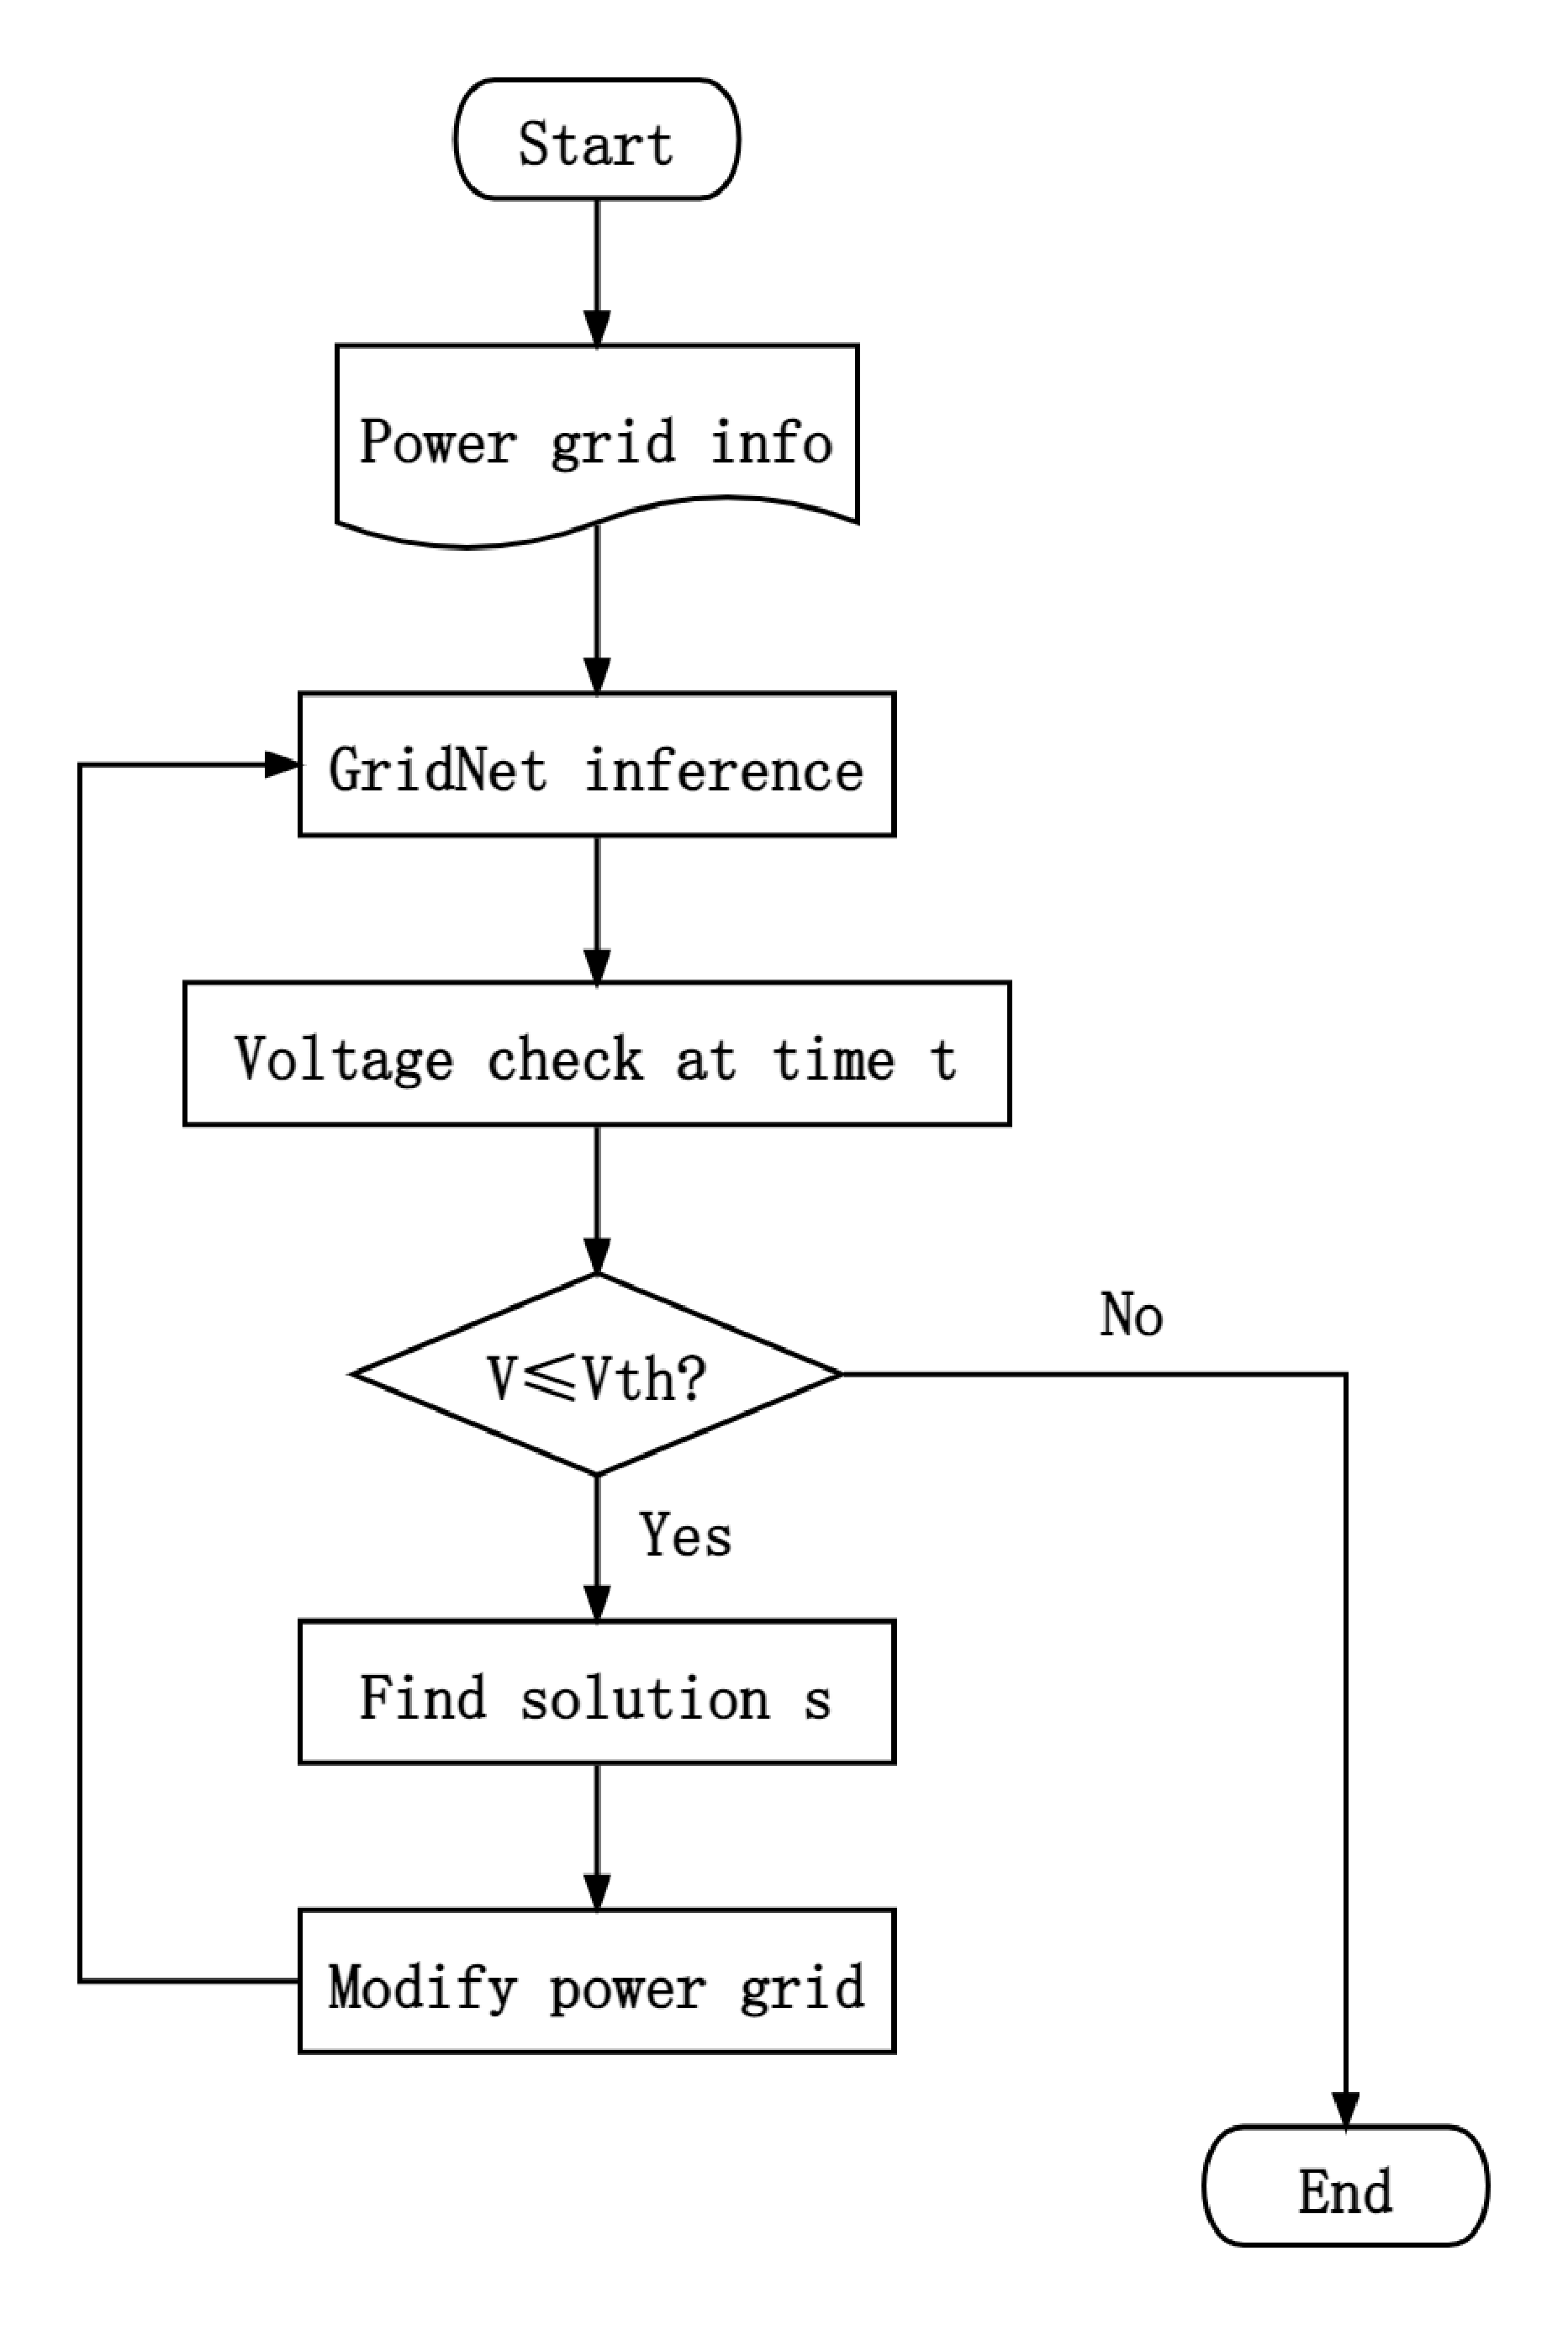
\includegraphics[width=0.7\columnwidth]{./figs/flowchart.eps}
%     \caption{The proposed strategy}
%     \label{fig:new_flowchart}
% \end{figure}

%\subsection{Conclude the algorithm}
%\label{subsec:algorithm}
% \subsection{Conjugate gradient optimization}
% As a comparison to our LP-based optimization strategy, we also enhance and implement ~\cite{ZhouJin:ICCAD'20}'s gradient-based localized fixing method to a globalized fixing method.  The localized fixing method in ~\cite{ZhouJin:ICCAD'20} will widen the power grid interconnect branches at the place of node voltage violation, the succeeding effect to node voltage is determined by the sensitivity matrix of node voltage to wire length acquired from the DNN prediction. Besides the localized power grid fixing, ~\cite{WuHong:2004TCAD}  and ~\cite{Fu:ASPDAC'05} have demonstrated that the globalized conjugate gradient-based method, which iteratively adds positive multiple of the last step direction to the steepest descent direction, can be applied on the on-chip IR drop and current density constrained optimization. But these methods are still analytically built on Black's EM model. Hence, we combine the idea of Fletcher-Reeves (F-R) conjugate gradient method and ~\cite{ZhouJin:ICCAD'20}'s sensitivity-based localized fixing method, and implement a globalized sensitivity-based conjugate gradient method in the power grid fixing optimization step as comparison. Simply speaking we utilize the conjugate gradient method to find out the branches which can maximize the node voltage fixing at the least cost of area increase. 

% We adopt a penalty function as follows:
% \begin{equation}\label{eq:penalty_f}
% f=a+p_{t}=a+\beta \cdot \sum _{j}c_{j,t}^{2}
% \end{equation}
% where $a$ is the network area, $p_{t}$ is the penalty term and $\beta$ is the penalty parameter, $c_{j,t}$ is the voltage drop for all the nodes with voltage violation.

% In this work, we utilize the Fletcher-Reeves (F-R) conjugate gradient method. The algorithm is shown as Algorithm~\ref{alg:pgvolopt}. The power grid is represented by the conductance matrix $G$.
% \begin{algorithm}[htbp]
% \caption{Conjugate gradient-based power grid fixing method}
% \label{alg:pgvolopt}
% \begin{algorithmic}[1]
% \renewcommand{\algorithmicrequire}{\textbf{Input:}}
% \renewcommand{\algorithmicensure}{\textbf{Output:}}
% \REQUIRE Original power grid $G$.
% \ENSURE New power grid $G$.
% % \STATE Set an initial value of penalty parameter $\beta$ and error bound $\varepsilon_{FR}$.
% \STATE Step $k:=0$.
% \STATE Set initial descent direction to negative direction of the gradient $P^{\left( k\right) }=-\nabla f$.
% %\REPEAT
% \WHILE{$\left\| \nabla f^{(k)} \right\|>\varepsilon$}
% 	\STATE Determine a positive $\lambda _{opt}^{\left( k\right) }$ that minimizes $f$.
% 	\STATE Update the power grid  $G^{\left( k+1\right) }=G^{\left( k\right) }+\lambda _{opt}^{(k)}P^{\left( k\right) }$.
% 	\STATE Deflect the descent direction $P^{\left( k+1\right)} = -\nabla f^{(k+1)} + \dfrac{\left\| \nabla f^{(k+1)}\right\| ^{2}}{\left\| \nabla f^{(k)} \right\| ^{2}} P^{\left( k\right)}$.
% 	\STATE $k:=k+1$.
% %\UNTIL{$\left\| \nabla f\left( G^{\left( k\right) }\right) \right\| <\varepsilon_{FR}$}
% \ENDWHILE
% \end{algorithmic}
% \end{algorithm}


\subsection{Fast sensitivity acquisition from back propagation}
\label{sec:new_VAEframework}
Instead of using the matrix solving method mentioned in section~\ref{subsec:exist_pgfix} to compute the sensitivity, we apply the machine learning strategy to fast acquire the sensitivity . First we train the VAE model extracted from the analytical results from $\it{EMspice}$, which provides the node voltage and branch resistance information of the power grid from $T = 0$ to $T = T_{target}$. 
The structure of the combined VAE and enhanced $\it{EMspice}$ analysis of the proposed strategy is shown in Fig.~\ref{subfig:flow-framework}. The workflow is concluded in Fig.~\ref{subfig:flow}. 

The output of the VAE mode contains two parts, the first part is the power grid nodes voltage at the target aging time considering the EM-induced aging effect, the second part is the sensitivity(gradient) of the output (voltage) with respect to the inputs (such as the resizing factor $s_{k}$ for the $k_{th}$ tree).  Such gradient acquisition can be very efficient as we can compute all the sensitivities just by one back propagation, and all the local gradients have been computed already. The acquirement of such sensitivity in our method utilizes the inherent characteristics of the differentiable VAE model. Once the models have been trained, they have the promise to be applied to the different designs, specially by using localized training as shown in recent work~\cite{WenPan:SemiTherm'2020}. 



\begin{figure*}[h!]
	\centering
	\captionsetup{justification=centering, margin=3cm}
	\subfigure[]{
		\includegraphics[width=1.207\columnwidth]{./figs/flow.eps}
		\label{subfig:flow-framework}}
	\subfigure[]{
		\includegraphics[width=0.74\columnwidth]{./figs/workflow-gridnetslp.eps}
		\label{subfig:flow}}
	\caption{The proposed (a)framework of  VAE-accelerated power gird fixing method (b) workflow of the fixing method.}
	\label{fig:flow}
\end{figure*}





\subsection{VAE-based model and training}
\label{subsec:dnn_training}


%The Generative Adversarial Network (GAN) is a form of neural network model utilized in unsupervised machine learning, originally developed by Ian Goodfellow. A standard GAN consists of two distinct deep neural networks - the generator G and the %discriminator D. G is tasked with producing outputs closely resembling the dataset used for training, whereas D is responsible for discerning between actual and artificially generated data. The generator within a typical GAN employs a random noise vector z as %its input, converting it to output G(z). The discriminator, a deep binary classifier, accepts both genuine and manufactured data alternately, offering a "score". This score is the basis for classifying data as "authentic" or "synthetic", and is also a component of the %loss function, used to train both G and D through back propagation. Training both networks is conducted concurrently and alternately to avoid one trailing significantly behind the other until equilibrium is achieved. In comparison, a regular Convolutional Neural %Network (CNN) utilizes a simple least square loss function, whereas the loss function of a GAN is a combination of the least square loss between prediction and actual data, and a discriminator's score. Thus, a GAN can be perceived as an advanced CNN with %improved accuracy.

%The Conditional Generative Adversarial Network (CGAN) operates within conditional settings, learning a conditional generative model. In contrast to a standard GAN, the generator's input in a CGAN is a fusion of both a condition vector x and a random noise %vector z, with the output labelled as G(x, z). The fundamental disparity with GAN lies in the fact that both G and D in a CGAN are conditional on vector x. CGANs have demonstrated outstanding performance in image-to-image translation tasks, where the input %image acts as the condition, directing the image generation process. In our study, the EM stress distribution generated is contingent on the input current density and given aging time, following the physics-law of stress evolution, making the CGAN model %exceptionally suitable.

Variational Autoencoders (VAEs) are a type of generative model, which are used to generate new data that is similar to the input data they're trained on.  VAEs have a unique architecture and learning procedure, compared to traditional autoencoders and GANs.
The traditional autoencoder structure includes encoder and decoder structures. A input will be encoded to a determined latent variable by the encoder, and then decoded to the output by the decoder. 
In VAE, the input is not directly encoded to a latent variable, instead its encoded to a distribution (usually multivariate Gaussian distribution) over the latent space,  and then re-samples latent variables from this distribution to generate a latent variable for the decoder. This re-sampling step is crucial to the VAE's some crucial characteristics over GANs, such as Interpretability of Latent Space, and Training Stability.
Interpretability of Latent Space means that the latent space is smooth and interpretable, enabling nice properties like the ability to interpolate between different points in the latent space and generate new samples that exhibit a smooth transition between the characteristics of the original points. On the other hand, GANs do not explicitly enforce such a structure, making the latent space less interpretable and interpolations might not always produce meaningful outputs. 

The Loss function for a VAE has two parts. The first is the reconstruction loss, which encourages the decoded data to be similar to the input data. The second is the KL divergence between the distribution output by the encoder and a prior (typically a standard Gaussian), which acts as a regularization term to encourage the network to use the latent space efficiently.  During training, the VAE learns to map the input data to a lower-dimensional latent space in a way that it can generate similar data from points in this space. Because of the probabilistic nature of the encoding, and the use of the KL divergence in the loss function, the VAE is encouraged to create a smooth and continuous latent space, where similar points decode to similar data.
\begin{figure*}[h!]
 \centering
 \includegraphics[width=1.8\columnwidth]{./figs/VAE_temp.eps}
\caption{The VAE model structure in our method} 
\label{fig:VAE_architecture}
\end{figure*}

The VAE model contain four convolutional layers and two fully-connected layers. The input is first padded to the standard size of 64 x 64 for the power grid smaller than this size. If the power grid exceeds the size of 64 x 64 but smaller than 128 x 128, then we add one more convolutional layer in both the generator and the discriminator network. For the further larger or smaller sized power grid, we follow the same routine to add or remove the convolutional layers to fit the input size.


As for our VAE-based model training, first we extract the electrical information from the result of the enhanced $\it{EMspice}$. The input features of VAE model should include the node voltage $u(t)$ and $M(t)$,  the conductance matrix of the power grid network in the format of wire segment resistance vectors, which are mentioned in Eq.~\eqref{eq:mna}. 
Suppose we are given a mesh-structured power grid network with proper topological and electrical information, the wire segment resistance can be derived from the wire length and segment width. The segment width of the mesh-structured power grid is proportional to the cross-sectional area. The trained VAE model will have the ability to predict different mesh-structured networks under same power grid topology. 

The data preprocessing before the model training is as follows. Synopsys IC compiler can automatically create the circuit layout from a synthesized gate-level netlist and a standard cell library. 
Then we parse the electrical features and the topological information from the circuit layout.


\begin{table}[!htbp]
	\begin{center}
		\caption{Power Grid Design Detail}
		\label{table:pre_results}
		%\vspace{-0.1in}
		\center
		\resizebox{0.48\textwidth}{!}{
		\begin{tabular}{ c | c | c | c | c}
			\hline 
			circuit &{\# nodes}&{\# Trees}&{\# voltage sources} &{$V_{DD}$ (V)}  \\ \hline 
			\hline 
			Design1 &1024 &64   &4 &1.05  \\ \hline
			Design2 &4096 &128  &4 &1.05 \\ \hline
			Design3 &16384 &256 &4 &1.05  \\ \hline
		\end{tabular}
		}
	\end{center}
	\vspace{-0.1in}
\end{table}


\begin{table}[!h]
	\begin{center} 
		\caption{Prediction results of VAE model and GAN model on different designs}
		\label{table: Model_RMSE_Compare}
		\center
			\begin{tabular}{| c| c | c | c | }
				\hline 
				{} &{} &\multicolumn{2}{c|} {RMSE (mV)}  \\
				\cline{3-4}
				\multirow{-2}{*}{Circuit}   &\multirow{-2}{*}{\# nodes} &{ GAN}  &{ VAE}   \\ \hline 
				\hline 
				Design1  &1024      &5.697 	& 3.144 	 \\ \hline
				Design2  &4096      &6.100	&  3.519	\\ \hline
				Design3  &16384   &3.922	        &  3.462	\\ \hline			
			\end{tabular}
	\end{center}
	\vspace{-0.1in}
\end{table}






\subsection{Sensitivity computation}
\label{subsec:new_sensivity}
We utilize the auto differentiation to calculate the sensitivity of output node voltage to the input power grid wire segment resistance, as VAE models are differentiable with respect to the model parameters.
  We use tensorflow.gradients API to compute such sensitivity in back-propagation of the generator network. 
The sensitivity information we obtained is organized in the following $n \times n_{t}$ \textit{Jacobian} matrix:
\begin{equation}
\label{eq:partial_jacob}
\mathbf J(t, s^{(r)})  =
\begin{bmatrix}
\frac{\partial v(t, s^{(r)})}{\partial s_{1}}&\frac{\partial v(t, s^{(r)})}{\partial s_{2}}&\ldots&\frac{\partial v(t, s^{(r)})}{\partial s_{n_{t}}}\\
\frac{\partial v(t, s^{(r)})}{\partial s_{1}}&\frac{\partial v(t, s^{(r)})}{\partial s_{2}}&\ldots&\frac{\partial v(t, s^{(r)})}{\partial s_{n_{t}}}\\
\vdots&\vdots&\ddots&\vdots\\
\frac{\partial v(t, s^{(r)})}{\partial s_{1}}&\frac{\partial v(t, s^{(r)})}{\partial s_{2}}&\ldots&\frac{\partial v(t, s^{(r)})}{\partial s_{n_{t}}}
\end{bmatrix}
\end{equation}
The resizing factor $s$ is updated, at each time step $r$.  Each column in the \textit{Jacobian} matrix describes how the node voltage will change due to the width rescaling of the corresponding power grid tree.
Then the \textit{Jacobian} matrix will be brought into  \eqref{eq:v_taylor_expand} to solve the linear programming problem. 
Notice that in the conventional circuit matrix method, each column in the \textit{Jacobian} matrix need to be calculated through the entire process mentioned in \eqref{eq:dVs}. In comparison our VAE-based method constructs the \textit{Jacobian} matrix by conducting the inference procedure only once.

%\begin{equation}
%\label{eq:partial_jacob}
%	J(t,s^{(r)}) \triangleq [\dfrac{\partial
%         v(t,s^{(r)})}{\partial s_{1}},
%        \dfrac{\partial v(t,s^{(r)})}{\partial s_{2}}, \ldots,
%        \dfrac{\partial v(t,s^{(r)})}{\partial s_{n_{t}}}]
%\end{equation}

% then \textit{Jacobian} matrix has to be entirely re-calculated by
% repeating the computation in \eqref{eq:dVs} for all trees, which
% consumes lots of time. 

% The \textit{Jacobian}
% matrix computation take more time when there is large amount of
% voltage violations and thereby a large amount of trees need
% resizing.

